\documentclass[12pt]{article}
\usepackage{amsmath,amssymb,relsize,enumitem,fancyhdr,parskip, pgfplots}
\usepackage{amsthm}
\usepackage[margin=1in]{geometry}
\usepackage{CJKutf8}
\newcommand{\Z}{\mathbb{Z}}
\newcommand{\R}{\mathbb{R}}
\newcommand{\N}{\mathbb{N}}
\theoremstyle{definition}
\newtheorem{definition}{Definition}[section]
\setlength{\headheight}{28pt}
\pgfplotsset{compat=1.16}
\pagestyle{fancy}
\fancyhf{}
\setlength{\parindent}{0pt}
\fancyhead[c]{Probabilistic and Combinatorial Analysis of Rainbow Board Refresh in \begin{CJK}{UTF8}{min}パズドラ\end{CJK}}
\fancyfoot[c]{\thepage}
        
\begin{document}
\tableofcontents
\section{Introduction}
Consider the standard $6\times 5$ (6 columns, 5 rows) board in the popular mobile game \begin{CJK}{UTF8}{min}パズドラ\end{CJK}. If you apply a rainbow board refresh (assuming all six standard orbs are equally probable), what is the probability of $i$ matches (including skyfalls), for $i\in\N$?
This is a deceptively hard problem as far as I can tell. I hope there is a nice closed form solution, but there probably isn't since it seems to involve partitioning.

Consider the problem with skyfalls disabled.
This limits the number of matches to $i=0,1,\dots,10$.

To consider skyfalls, we may consider the boards as states of a Markov chain (maybe). The expected 

\section{$2\times2$ board with 2-matches}
\subsection{Initial board}
Consider a simplification of the problem.
The board is now $2 \times 2$, and a match occurs when at least two orbs are adjacent (non-diagonal) to each other.

It is not hard to enumerate all of the $6^4=1296$ possible boards, grouping them by resultant combos and board configuration.
\begin{itemize}
    \item 0 combos
    \begin{itemize}
        \item Each of the four orbs are distinct colors, so there are $\binom{6}{4}\cdot 4!=360$ boards
        \begin{center}
            \begin{tabular}{|c|c|}
            \hline
            a & b \\
            \hline
            c & d \\
            \hline
            \end{tabular}
        \end{center}
        This probability is $360/1296=5/18$.
        \item Two of the four orbs are the same color. In order to avoid matches, the two same-colored orbs are diagonal from each other. Therefore there are two possibilities.
        \begin{center}
            \begin{tabular}{|c|c|}
            \hline
            a & b \\
            \hline
            c & a \\
            \hline
            \end{tabular}
            \qquad
            \begin{tabular}{|c|c|}
            \hline
            b & a \\
            \hline
            a & c \\
            \hline
            \end{tabular}
        \end{center}
        This results in $2\cdot\binom{6}{3}\cdot 3!=240$ boards.
        This probability is $240/1296=5/27$.
        \item Two orbs are the same color and the remaining two orbs are both the same different color. To avoid matches, the same-color pairs must be diagonal from each other, and there is only a single case.
        \begin{center}
            \begin{tabular}{|c|c|}
            \hline
            a & b \\
            \hline
            b & a \\
            \hline
            \end{tabular}
        \end{center}
        This results in $\binom{6}{2}\cdot 2!=30$ boards.
        This probability is $30/1296=5/216$.
    \end{itemize}
    In total, the probability of 0 combos is $(360+240+30)/1296=35/72$.
    \item 1 combo
    \begin{itemize}
        \item With three colors, we can have the following possibilities:
        \begin{center}
            \begin{tabular}{|c|c|}
            \hline
            a & b \\
            \hline
            a & c \\
            \hline
            \end{tabular}
            \quad
            \begin{tabular}{|c|c|}
            \hline
            a & a \\
            \hline
            b & c \\
            \hline
            \end{tabular}
            \quad
            \begin{tabular}{|c|c|}
            \hline
            b & c \\
            \hline
            a & a \\
            \hline
            \end{tabular}
            \quad
            \begin{tabular}{|c|c|}
            \hline
            b & a \\
            \hline
            c & a \\
            \hline
            \end{tabular}
        \end{center}
        This results in $4\cdot \binom{6}{3}\cdot 3!=480$ boards.
        \item WIth two colors, we have the following possibilities:
        \begin{center}
            \begin{tabular}{|c|c|}
            \hline
            a & a \\
            \hline
            a & b \\
            \hline
            \end{tabular}
            \quad
            \begin{tabular}{|c|c|}
            \hline
            a & a \\
            \hline
            b & a \\
            \hline
            \end{tabular}
            \quad
            \begin{tabular}{|c|c|}
            \hline
            b & a \\
            \hline
            a & a \\
            \hline
            \end{tabular}
            \quad
            \begin{tabular}{|c|c|}
            \hline
            a & b \\
            \hline
            a & a \\
            \hline
            \end{tabular}
        \end{center}
        This results in $4\cdot \binom{6}{2}\cdot 2!=120$ boards.
        \item 
        If all four orbs are the same color, there is only one configuration and $6$ possible boards.
    \end{itemize}
    In total, the probability of 1 combo is $(480+120+6)/1296=101/216$.
    \item 2 combo
    \begin{itemize}
        \item Two adjacent orbs are the same color, and the other two adjacent orbs are another same color.
        \begin{center}
            \begin{tabular}{|c|c|}
            \hline
            a & b \\
            \hline
            a & b \\
            \hline
            \end{tabular}
            \qquad
            \begin{tabular}{|c|c|}
            \hline
            a & a \\
            \hline
            b & b \\
            \hline
            \end{tabular}
        \end{center}
        This results in $2\cdot\binom{6}{2}\cdot 2!=60$ boards.
    \end{itemize}
    The probability of 2 combos is $60/1296=5/108$.
\end{itemize}
\begin{center}
\begin{tikzpicture}
\begin{axis}[
    title=Initial Distribution,
	ylabel=Probability,
	ymax=1,
	enlargelimits=0.15,
	ybar,
	xtick=data,
	xlabel=Combos
]
\addplot coordinates {(0, 35/72) (1, 101/216) (2, 5/108)};
\end{axis}
\end{tikzpicture}
\end{center}
This distribution is consistent with Monte Carlo simulations.
\subsection{Skyfalls enabled}
Now we can consider the board configurations as states of a discrete-time stochastic process. The first thing we should figure out is if this process is Markovian. (Of course it is, since all predictive information about future combos is obtained by the current state of the board.) Another thing to consider is the fact that the number of combos is unbounded when skyfalls are enabled, but the expected number of combos is (probably?) finite.

The best way to assign states is probably the distinct board configurations as listed above.

\begin{itemize}
    \item 0 combo
    \begin{itemize}
        \item Clearly the boards with 0 matches/combos are absorbing states as they do not give rise to any skyfalls, let alone skyfall combos. Any prior board information does not impact the future states since there cannot be any skyfalls.
    \end{itemize}
    \item 1 combo
    \begin{itemize}
        \item The three color case leads to three distinct possible remainder boards.
        \begin{center}
            \begin{tabular}{|c|c|}
            \hline
             &  \\
            \hline
            a & b \\
            \hline
            \end{tabular}
            \qquad
            \begin{tabular}{|c|c|}
            \hline
            a & \phantom{a} \\
            \hline
            b & \phantom{a} \\
            \hline
            \end{tabular}
            \qquad
            \begin{tabular}{|c|c|}
            \hline
            \phantom{a} & a \\
            \hline
            \phantom{a} & b \\
            \hline
            \end{tabular}
        \end{center}
        The first board occurs with conditional probability $1/2$, while the other two each occur with probability $1/4$.
        
        What are the possible boards after skyfall? Find out on the next episode...
        \item 
        The two color case with a single combo results in a single remainder orb at the lower left or lower right, each with equal probability. The color of the remainder orb is known, but no other information about the board configuration is known. Therefore all of the initial boards, restricted to those with the appropriate color assignments are possible. That is, we think about all the possible boards and divide by six to exclude those with the inconsistent remainder orb.
        \item The single color case is equivalent to a complete board refresh. Therefore all of the initial boards are once again equally likely. Prior information about the board is irrelevant.
    \end{itemize}
    \item 2 combo
    \begin{itemize}
        \item All of the orbs are cleared, so the initial boards are all equally likely. Prior information about the board is irrelevant.
    \end{itemize}
With this information, let $x$ be the expected number of combos, including those contributed by skyfalls. Then we have
\begin{align*}
    x = 0(35/72) + (101/216)(1+x) + (5/108)(2+x)
    \implies x = 121/105
\end{align*}
Thus the theoretical expected number of combos is 121/105.

Next step: Confirm or deny using simulation.

Luckily cascades are not possible in a $2\times 2$ board, otherwise analysis would be insanely difficult.
\end{itemize}
\subsection{Poison, mortal poison, jammer, bomb orbs enabled}
What if we want to consider more than just the six standard orb colors? If we generalize to $c$ colors, the number of boards increases to $c^4$ boards. However, the same analysis of board configurations as before works, replacing all instances of 6 with $c$, as long as $c\geq 2\times 2$. If $c<4$, then the possible board configurations changes, along with their associated probabilities.

For $c\geq 4$, we find the distribution for the initial board. Applying the same analysis as above results in the following:
\begin{center}
    \renewcommand{\arraystretch}{2}
    \begin{tabular}{|c|c|}
        \hline
        Number of Combos & Probability \\
        \hline\hline
        0 & $\left[\binom{c}{4}\cdot 4! + 2 \cdot \binom{c}{3}\cdot 3! + \binom{c}{2} \cdot 2!\right]/c^4$\\
        \hline
        1 & $\left[4\cdot \binom{c}{3}\cdot 3!+4\cdot\binom{6}{2}\cdot 2! + c\right]/c^4$ \\
        \hline
        2 & $\left[2\cdot\binom{c}{2}\cdot 2!\right]/c^4$\\
        \hline
    \end{tabular}
    \renewcommand{\arraystretch}{2}
\end{center}
Keep in mind this also assumes the $c$ different orb colors are assumed to be equally probable. Otherwise, the problem gets even more complicated.


\section{$6\times 5$ board with 3-matches}
We return to the classical problem on a $6\times 5$ board, allowing 3-matches.

\subsection{Classifying boards based on number of colors}

Here we count all the boards with exactly $i$ number of colors for $i=1,\dots,6$ and compute the probabilities of occurrence after a random board refresh. Note that the total number of boards is $6^{5\times 6}=6^{30}$.

If a board is monocolor, there are $\binom{6}{1}$ boards, since we choose one color from the possible six. Thus the probability of occurrence is $\binom{6}{1}/6^{30}$.

How many distinct bicolor boards are there? Since we can choose two out of six colors and one of the two colors for each orb, there are $\binom{6}{2}\cdot 2^{30}$ boards with at most two colors. This includes all of the monocolor boards, so number of strictly bicolor boards is $\binom{6}{2}\cdot 2^{30}-\binom{6}{1}$.

In a similar fashion, the number of boards with exactly $i$ colors is $\binom{6}{i}\cdot i^{30}-\binom{6}{i-1}\cdot (i-1)^{30}$. The probability of having a board with $i$ colors is $\left[\binom{6}{i}\cdot i^{30}-\binom{6}{i-1}\cdot (i-1)^{30}\right]/6^{30}$.

\begin{center}
\renewcommand{\arraystretch}{2}
    \begin{tabular}{|c|c|c|}
        \hline
        Number of Colors & Number of Boards & Approximate Probability \\
        \hline\hline
        $1$ & $\binom{6}{1}$ & $%\binom{6}{1}/6^{30}\approx 
        2.71\times 10^{-23}$ \\
        \hline
        $2$ & $\binom{6}{2}\cdot 2^{30}-\binom{6}{1}$ & $%\left[\binom{6}{2}\cdot 2^{30}-\binom{6}{1}\right]/6^{30}\approx
        7.29\times 10^{-14}$ \\
        \hline
        $3$ & $\binom{6}{3}\cdot 3^{30}-\binom{6}{2}\cdot 2^{30}$ & $%\left[\binom{6}{3}\cdot 3^{30}-\binom{6}{2}\cdot 2^{30}\right]/6^{30}\approx 
        1.86\times 10^{-8}$ \\
        \hline
        $4$ & $\binom{6}{4}\cdot 4^{30}-\binom{6}{3}\cdot 3^{30}$ & $%\left[\binom{6}{4}\cdot 4^{30}-\binom{6}{3}\cdot 3^{30}\right]/6^{30}\approx 
        7.82\times 10^{-5}$ \\
        \hline
        $5$ & $\binom{6}{5}\cdot 5^{30}-\binom{6}{4}\cdot 4^{30}$ & $%\left[\binom{6}{5}\cdot 5^{30}-\binom{6}{4}\cdot 4^{30}\right]/6^{30}\approx 
        2.52\times 10^{-2}$ \\
        \hline
        $6$ & $\binom{6}{6}\cdot 6^{30}-\binom{6}{5}\cdot 5^{30}$ & $%\left[\binom{6}{6}\cdot 6^{30}-\binom{6}{5}\cdot 5^{30}\right]/6^{30}\approx 
        0.975$ \\
        \hline
    \end{tabular}
\renewcommand{\arraystretch}{2}
\end{center}
These exact probabilities indicate that it is extremely likely to end up with a board containing five or six colors, while monocolor, bicolor, tricolor, and quadcolor boards almost never occur. 

\begin{definition}
    A board is called \textbf{rainbow matchable} if it contains at least 3 orbs of each color.
\end{definition}

A few natural questions arise:
\begin{enumerate}
    \item Unconditionally (that is, a board with or without preexisting matches), what is the probability that the board is rainbow matchable?
    \item Given a 0 combo board, what is the probability that the board is rainbow matchable.?
\end{enumerate}
At first glance, the answer to these two problems might seem like they should be identical. However, maybe it is possible that 0 combo boards increase (or decrease) the likelihood because some configurations are favored. For example when considering 0 combo boards, monocolor boards are excluded entirely, and the majority of bicolor and tricolor boards are excluded as well.
\subsection{Classifying monocolor boards}
There are only six of them, each resulting in another board refresh. This subsection is only included for completeness.
\subsection{Classifying bicolor boards}
We know there are $\binom{6}{2}\cdot 2^{30}-\binom{6}{1}$ bicolor boards from earlier.

If we fix the two colors, there are only $2^{30}-2$ distinct board configurations. ???
% Am I somehow miscounting? Because there is symmetry between two colors
\subsection{Average number of natural explicit combos}
Natural means all distinct boards are equally likely. Explicit means no implicit combos due to skyfalls or cascades.

After doing Monte Carlo simulation with 10 million trials, we find the average number of combos is approximately 0.8557792.

The approximate distribution is as follows:
\begin{center}
\begin{tabular}{|c|c|}
    \hline
    Combos & Approximate Probability \\
    \hline\hline
    0 combos & 0.3793952 \\
    \hline
    1 combo & 0.422572 \\
    \hline
    2 combos & 0.1651948 \\
    \hline
    3 combos & 0.0299233 \\
    \hline
    4 combos & 0.0027802 \\
    \hline
    5 combos & 0.000132 \\
    \hline
    6 combos & 0.0000025 \\
    \hline
    7 combos & 0 \\
    \hline
    8 combos & 0 \\
    \hline
    9 combos & 0 \\
    \hline
    10 combos & 0 \\
    \hline
\end{tabular}
\end{center}
\begin{center}
\begin{tikzpicture}
\begin{axis}[
    title=Simulated Initial Distribution,
	ylabel=Probability,
	ymax=1,
	enlargelimits=0.15,
	ybar,
	xtick=data,
	xlabel=Combos
]
\addplot coordinates {(0, 0.3793952) (1, 0.422572) (2, 0.1651948) (3, 0.0299233) (4, 0.0027802) (5, 0.000132) (6, 0.0000025) (7, 0) (8, 0) (9, 0) (10, 0)};
\end{axis}
\end{tikzpicture}
\end{center}
The exact values? Find out on the next episode of \textit{Cases: The Adventure}.
\section{$m\times n$ board with $k$-matches}
I don't know if this is even possible to study further than running a few Monte Carlo simulations. Combinatorics is hard.
\end{document}